\documentclass{beamer}
\usepackage[T1]{fontenc}
\usepackage[utf8]{inputenc}
\usepackage{lmodern}
\usepackage{ngerman}
\usepackage{graphics}
\usepackage{amsmath}
\usetheme{Singapore}
\usecolortheme{dove}
\graphicspath{{images/}{../comics/}}
\newcommand{\hiddencell}[2]{\action<#1->{#2}}

\title{Grundbegriffe der Informatik}
\author{Patrick Niklaus}

\begin{document}
\begin{frame}
  \frametitle{Grundbegriffe der Informatik}
  \framesubtitle{2. Tutorium}
  \begin{description}
    \item \textbf{Name:} Patrick Niklaus
    \item \textbf{E-Mail:} patrick.niklaus@student.kit.edu
    \item \textbf{Nr:} 43
  \end{description}
\end{frame}

\section{Wörter}
\subsection{Alphabete}
\begin{frame}
  \frametitle{Alphabete}
  \begin{definition}
    Sei A eine endliche Menge von Symbolen. Dann heißt A ein \emph{Alphabet}.
  \end{definition}
  \begin{exampleblock}{Beispiele}
    \begin{itemize}
      \item $A := \{a, b, c\}$
      \item $A := \{\phi, 1, 2\}$
      \item $A := \{l, r, t, o\}$
    \end{itemize}
  \end{exampleblock}
\end{frame}
\subsection{Wörter}
\begin{frame}
  \frametitle{Wörter}
  \begin{definition}
    Sei A ein Alphabet und $w: \mathbb{G}_n \rightarrow A$ eine \emph{surjektive} Abbildung. Dann heißt w ein \emph{Wort über dem Alphabet A}.
  \end{definition}\pause
  \begin{alertblock}{Etwas weniger formal}
    Ein Wort ist eine Folge von Symbolen aus einem Alphabet A.
  \end{alertblock}\pause
  \begin{definition}
    Das Wort $\varepsilon: \{\} \rightarrow \{\}$ heißt das \emph{leere Wort}. \\
    {\tiny Neutrales Element gegenüber der Wortkonkatenation.}
  \end{definition}\pause
  \begin{alertblock}{Erinnerung}
    $\mathbb{G}_n :=  \{k \in \mathbb{N}_0 | 0 \leq k < n\} \Rightarrow \mathbb{G}_0 = \{\}$
  \end{alertblock}
\end{frame}
\begin{frame}
  \frametitle{Wörter}
  \begin{exampleblock}{Beispiele}
    \begin{itemize}
      \item
      $
        w_1: \mathbb{G}_5 \rightarrow \{l, r, t, o\}: w_1(i) \mapsto \left\{
        \begin{array}{l l}
          t, & \quad i = 0\\
          r, & \quad i = 1\\
          l, & \quad i \in \{2, 4\}\\
          o, & \quad i = 3\\
        \end{array} \right.
      $ \\
      wir schreiben auch $w_1 = trlol$
      \item
      $
        w_2: \mathbb{G}_6 \rightarrow \{1, 0\}: w_2(i) \mapsto \left\{
        \begin{array}{l l}
          1, & \quad \text{$i$ gerade}\\
          0, & \quad \text{$i$ ungerade}\\
        \end{array} \right.
      $ \\
      wir schreiben auch $w_2 = 101010$
    \end{itemize}
  \end{exampleblock}
\end{frame}
\subsection{Konkatenation}
\begin{frame}
  \frametitle{Konkatenation von Wörtern}
  \begin{definition}
    Seien $w_1: \mathbb{G}_{n_1} \rightarrow A_1, w_2: \mathbb{G}_{n_2} \rightarrow A_2$ Wörter.\\
    Dann ist $w_1 \cdot w_2: \mathbb{G}_{n_1 + n_2} \rightarrow A_1 \cup A_2,$
    $(w_1 \cdot w_2)(i) \mapsto \left\{
        \begin{array}{l l}
          w_1(i), & \quad 0 \leq i < n_1\\
          w_2(i-n_1), & \quad n_1 \leq i < n_2\\
        \end{array} \right.
    $\\
    die Konkatenation von $w_1$ und $w_2$.
  \end{definition}\pause
  \begin{alertblock}{Etwas weniger formal}
    Wir hängen die Buchstabenfolge $w_1$ an $w_2$ an.
  \end{alertblock}
\end{frame}
\begin{frame}
  \frametitle{Konkatenation von Wörtern}
  \begin{exampleblock}{Beispiele}
    \begin{enumerate}
      \item $w_1 := ab, w_2 := ba$\\
             $w_1 \cdot w_2 = ab \cdot ba = abba$
      \item $w_1 := Hallo, w_2 := We, w_3 := lt$\\
             $w_1 \cdot w_2  \cdot w_3 = Hallo \cdot We \cdot lt = HalloWelt$
      \item $w_1 := 01$\\
             $w_1^3 = w_1 \cdot w_1^2 = w_1 \cdot w_1 \cdot w_1 = 10 \cdot 10 \cdot 10 = 101010$
    \end{enumerate}
  \end{exampleblock}
\end{frame}

\begin{frame}
  \frametitle{Menge aller Wörter}
  \begin{definition}
    Die Menge der Wörter der Länge \emph{n} wird bezeichnet mit $A^n$. Die Menge aller Wörter $A^*$ ist definiert als $A^* = \bigcup \limits^{\infty}_{i=0} A^i$ \emph{(Kleenesche Hülle von A)}.
  \end{definition}
  \begin{exampleblock}{Beispiele}
    \begin{enumerate}
      \item $A := \{a, b\}, A^3 = \{aaa, aab, aba, abb, baa, bab, bba, bbb\}$
      \item $A := \{0, 1\}, A^* = \{\varepsilon, 0, 1, 00, 11, 01, 10, 000, 001, ...\}$
      \item $A := \{a, b, c\}, A^* = \{\varepsilon, a, b, c, aa, ab, ac, bb, ba, ...\}$
    \end{enumerate}
  \end{exampleblock}
\end{frame}


\section{Formale Sprachen}
\subsection{Definitionen}
\begin{frame}
  \frametitle{Formale Sprachen}
  \begin{definition}
    Sei A ein Alphabet. $L \subseteq A^*$ heißt \emph{formale Sprache über dem Alphabet A}.
  \end{definition}\pause
  \begin{exampleblock}{Beispiele}
    \begin{itemize}
      \item $A := \{1, 0\}, L:= \{011, 101, 110\} \subset A^*$ \pause
      \item $A := \{a, b\}, L:= \{ab, abab, ababab, ababab, ...\} \subset A^*$ \pause
      \item $A := \{a, b\}, L:= \{ab, aabb, aaabbb, aaaabbbb, ...\} \subset A^*$
    \end{itemize}
  \end{exampleblock}
\end{frame}
\begin{frame}
  \frametitle{Produkt von Sprachen}
  \begin{definition}
    Seien $L_1, L_2$ formale Sprachen. Dann ist $L_1 \cdot L_2 := \{w_1 \cdot w_2 | w_1 \in L_1, w_2 \in L_2\}$ das Produkt von $L_1$ und $L_2$.
  \end{definition}\pause
  \begin{exampleblock}{Beispiele}
    \begin{itemize}
      \item $L_1 := \{a, aa\}, L_2 := \{bb, bbb\}$,\\
             $L_1 \cdot L_2 = \{abb, abbb, aabb, aabbb\}$ \pause
      \item $L_1 := \{20, 19\}, L_2 := \{10, 12\},$\\
             $L_1 \cdot L_2 = \{2010, 2012, 1910, 1912\}$\\
             $L_2 \cdot L_1 = \{1020, 1220, 1019, 1219\}$
    \end{itemize}
  \end{exampleblock}
  \begin{alertblock}{Nicht kommutativ!}
  \end{alertblock}
\end{frame}
\begin{frame}
  \frametitle{Potenzen von Sprachen}
  \begin{definition}
    Sei L eine formale Sprache. Dann ist $L^0 = \varepsilon, L^n := w_1 \cdot ... \cdot w_n$, (mit $w_1, ..., w_n \in L$) die \emph{n-te Potenz von L}.
  \end{definition}\pause
  \begin{exampleblock}{Beispiele}
    \begin{itemize}
      \item $L := \{ab, ba\}, L^3 := \{ababab, ababba, abbaab, abbaba, baabab, baabba, babaab, bababa\}$
      \item $L := \{a, b, c\}, L^2 := \{aa, ab, ac, ba, bb, bc, ca, cb, cc\}$
    \end{itemize}
  \end{exampleblock}
\end{frame}
\begin{frame}
  \frametitle{Konkatenationsabschluss von Sprachen}
  \begin{definition}
    Sei L eine formale Sprache. Die Menge aller Wörter, die sich aus Wörtern dieser Sprache L zusammen setzen lassen ist definiert als\\
    \begin{description}
      \item[Konkatenationsabschluss:] $L^* = \bigcup \limits^{\infty}_{i=0} L^i$.
      \item[$\varepsilon$-freier Konkatenationsabschluss:] $L^+ = \bigcup \limits^{\infty}_{i=1} L^i$.
    \end{description}
  \end{definition}\pause
  \begin{exampleblock}{Beispiele}
    \begin{itemize}
      \item $L := \{a0, b1, c2\}, L^* = \{\varepsilon, a0, b1, c2, a0a0, a0b1, ...\}$\\
             $L^+ = \{a0, b1, c2, a0a0, a0b1, ...\}$
      \item $L := \{00, 1\}, L^* = \{\varepsilon, 00, 1, 100, 001, ...\}$\\
             $L^+ = \{\varepsilon, 00, 1, 100, 001, ...\}$
    \end{itemize}
  \end{exampleblock}
\end{frame}

\subsection{Aufgaben}
\begin{frame}
  \frametitle{Aufgaben}
  \begin{exampleblock}{In Mengen M aus Studenten mit $|M| \leq 3$}
      Bestimmt folgende Sprachen in Mengenschreibweise:
      \begin{enumerate}
        \item $L_1$ sei die Sprache über $A := \{a, b\}$ bei der alle Worte mit a beginnen und nur ab-Teilworte folgen.
        \item $L_2 := \{ba\}^* \cdot \{ab\}^+$
      \end{enumerate}
      Bestimmt ob die angegebenen Worte in den entsprechenden Sprachen liegen:
      \begin{enumerate}
        \item $w_1 = \varepsilon, w_2 = ab, w_3 = abbaab, L_1 := \{\varepsilon\}^+ \cdot \{ab\} \cdot \{ba\}^*$
        \item $w_1 = \varepsilon, w_2 = ab, w_3 = abbaab, L_1 := \{aaa\}^* \cdot \{b\}^+ \cdot \{a\}^3$
      \end{enumerate}
  \end{exampleblock}
\end{frame}


\section{Abschluss}
\subsection{Zusammenfassung}
\begin{frame}
  \frametitle{Was ihr mitnehmen sollt}
  \begin{enumerate}
    \item Foo
   \end{enumerate}
\end{frame}

\subsection{xkcd}
\begin{frame}[plain]
  \begin{figure}
    \begin{center}
      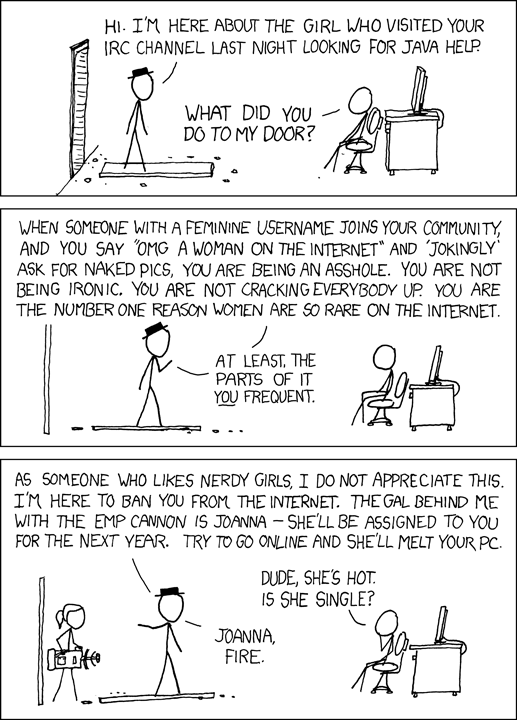
\includegraphics[height=250pt]{pix_plz}
    \end{center}
  \end{figure}
\end{frame}

\end{document}
